\documentclass[11pt]{article}
\usepackage[margin=1in]{geometry}
\usepackage{amsmath}
\usepackage{graphicx}
\usepackage{float}
\usepackage{placeins}

\title{Meeting}

\begin{document}
\maketitle
\section{Overview}
  \begin{itemize}
    \item As of our last meeting, we had seen that Chen's method didn't seem to perform well when we modified it to use our version of the premium. The method seemed to overfit fairly quickly. We also discussed the email I drafted to ask them clarification questions about how they processed their data. 
    \item I decided to try a few more things with regards to processing the data before sending the email, and I was able to resolve a lot of the discrepancies. What ended up making the biggest difference was using the difference method instead of the ratio method for detrending the yield time-series. I had initially used the ratio method because they didn't specify which one they used, and both papers they cited when discussing the detrending used the ratio method. Once I tried the difference method the yield values became a lot more similar. 
    \item I was also able to figure out why their method was overfitting. I had to play around with the network hyperparameters, but once I changed the learning rate the network was able to learn normally. 
    \item After changing the data and fixing their network, the results flipped. Chen's method outperformed ours in the full data setting, on average by $5\%$. Their method outperformed our regardless of the definition of the premium that was used. This is what we originally expected.  
    \item As a result, I decided to run the data shortening exercise, because we hypothesized that our method would perform better in data-scarce settings.  
  \end{itemize}

\section{Data Shortening Exercise}
  Earlier, we had hypothesized that our method should perform better in data scarce settings. The data scarce setting is also motivated by the developing country context. In Chen's paper, the data goes back to 1925. However, the large majority of developing countries don't have weather data going back that far. Many rely on historical satellite data, which, in the best circumstances, is available since 1970 or so. However, most satellite data became available in 1980 or 1990. 
  To test how the performance of the method changed as less data became available, we artificially shortened the data. We tested both methods with only 90 years of data available, 80 years, and so on until only 30 years of data were available. In all cases, we used a $70/15/15$ train, validation, test split (as specified in Chen et al 2023), using the later years for validation and testing. As before, we ran two sets of experiments, one using Chen's definition of the premium and one using our definition of the premium. In all cases, I compared our method to Chen's unconstrained method, because that's the one they reported results on. 

  \subsection{Results}
    In general, our method outperformed Chen's method when there was less than 70 years of data available. This held with both definitions of the premium. When there was 70 or more years of data available, Chen's method tended to do better. Although not as strong as before, I think this is still a good result. In practice, in the best cases there's usually 40-50 years of weather data available in developing countries. And in this domain, our method performs better. Additionally, our method provides a direct mapping of loss to payouts, which I think makes it more interpretable/useful for farmers and policy makers. 

  \subsubsection{Our definition of the premium}
  \begin{figure}[h]
    \centering
    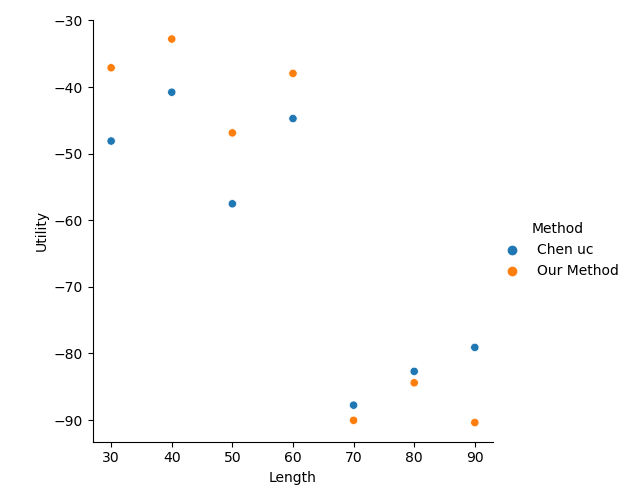
\includegraphics[width=0.6\textwidth]{../../../output/figures/Chen_Replication/Our_premium_results.png}
    \caption{Data shortening exercise using our definition of the premium. Here, Length is dataset length, or number of years of data available}
  \end{figure}
  \FloatBarrier
  \subsubsection{Chen's definition of the premium}
  \begin{figure}[h]
    \centering
    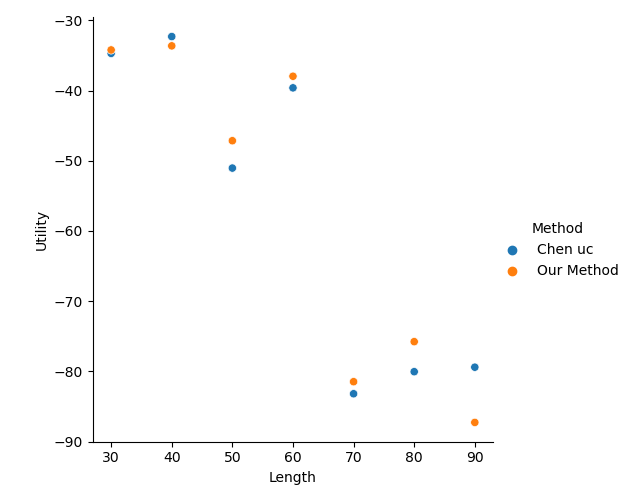
\includegraphics[width=0.6\textwidth]{../../../output/figures/Chen_Replication/chen_premium_results.png}
    \caption{Data shortening exercise using Chen's definition of the premium. Here, Length is dataset length, or number of years of data available}
  \end{figure}
  \FloatBarrier

\section{Next Steps}
  There are a couple of things we can add, I'm listing them in order of how much I think they would add to the paper. 
\begin{itemize}
  \item \textbf{Multiple Zones:} We could compare the cost of insuring the US midwest (Illinois, Indiana, Missouri, Iowa) under both methods. Given the difference in performance between the two methods in the full data setting, I'm not sure we'll outperform their method if we use the full data here. One option would be to add data shortening to this exercise. We could compare the cost of insuring the US midwest under both methods as less data becomes available. This could be motivated by our context, but I'm not sure if it would seem too contrived. Here, we would have to think about whether or not to keep the same min max objective as before, or to use a overall sum of utilities objective. 
  \item \textbf{Descriptive Analysis:} We could create plots to illustrate the difference between the two methods: 
    \begin{enumerate}
      \item Plot of payouts vs losses
      \item Distribution of farmer utility/wealth
      \item Distribution of insurer costs
      \item Distribution of insurer profits
      \item Plot illustrating in what cases farmer's are worse off with insurance
    \end{enumerate}
\end{itemize}
\end{document}